\section{Experimental Results and Analysis}
\label{sec:results}

This section reports the quantitative and spatial experimental results obtained from the UrbanVending AI pipeline, encompassing unsupervised spatial clustering, MCDA sensitivity analysis, Goal Programming optimization, physical micro-slot packing validation, and supervised suitability benchmarking with TreeSHAP explainability.

\subsection{Environmental Spatial Clustering Analysis}
\label{sec:res_clustering}

Fig.~\ref{fig:kmeans_before_after} illustrates the spatial clustering of the 258 usable zone geometries across Nashik before and after feature engineering and outlier normalization.

\begin{figure}[t]
    \centering
    \begin{minipage}{0.48\columnwidth}
        \centering
        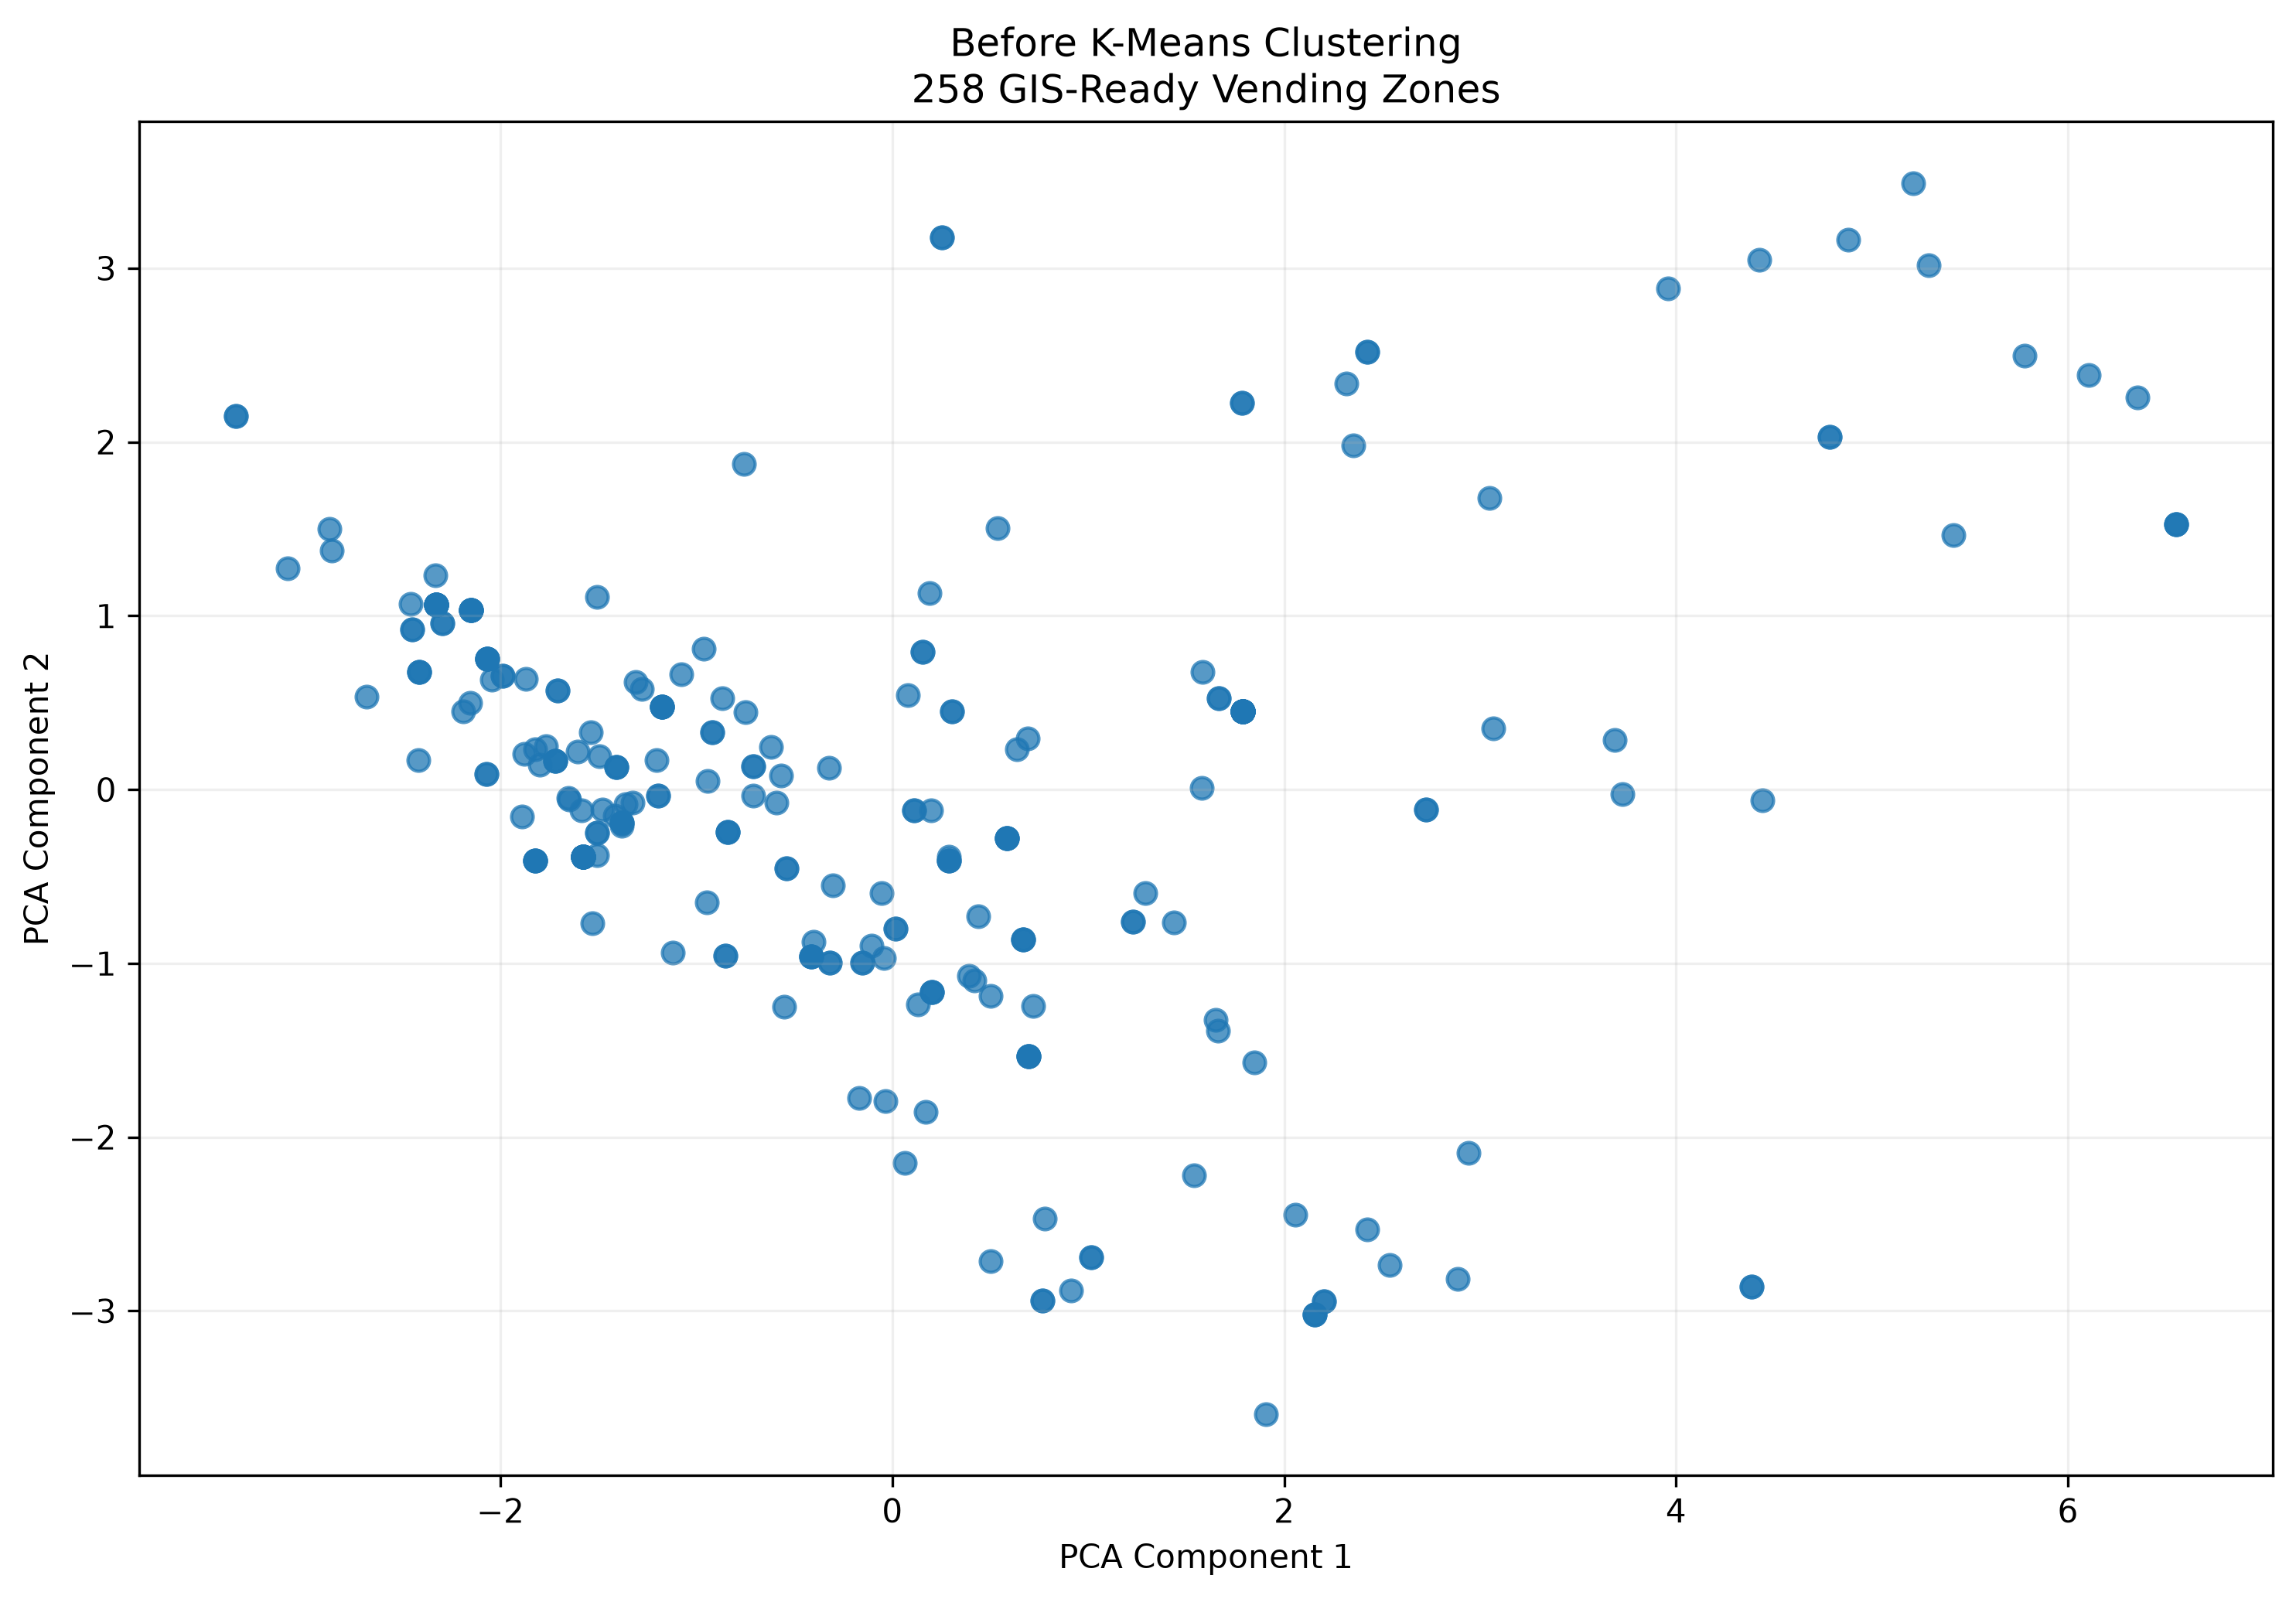
\includegraphics[width=\linewidth]{figures/kmeans_before.png}
        \caption*{(a) Before Feature Transformation}
    \end{minipage}\hfill
    \begin{minipage}{0.48\columnwidth}
        \centering
        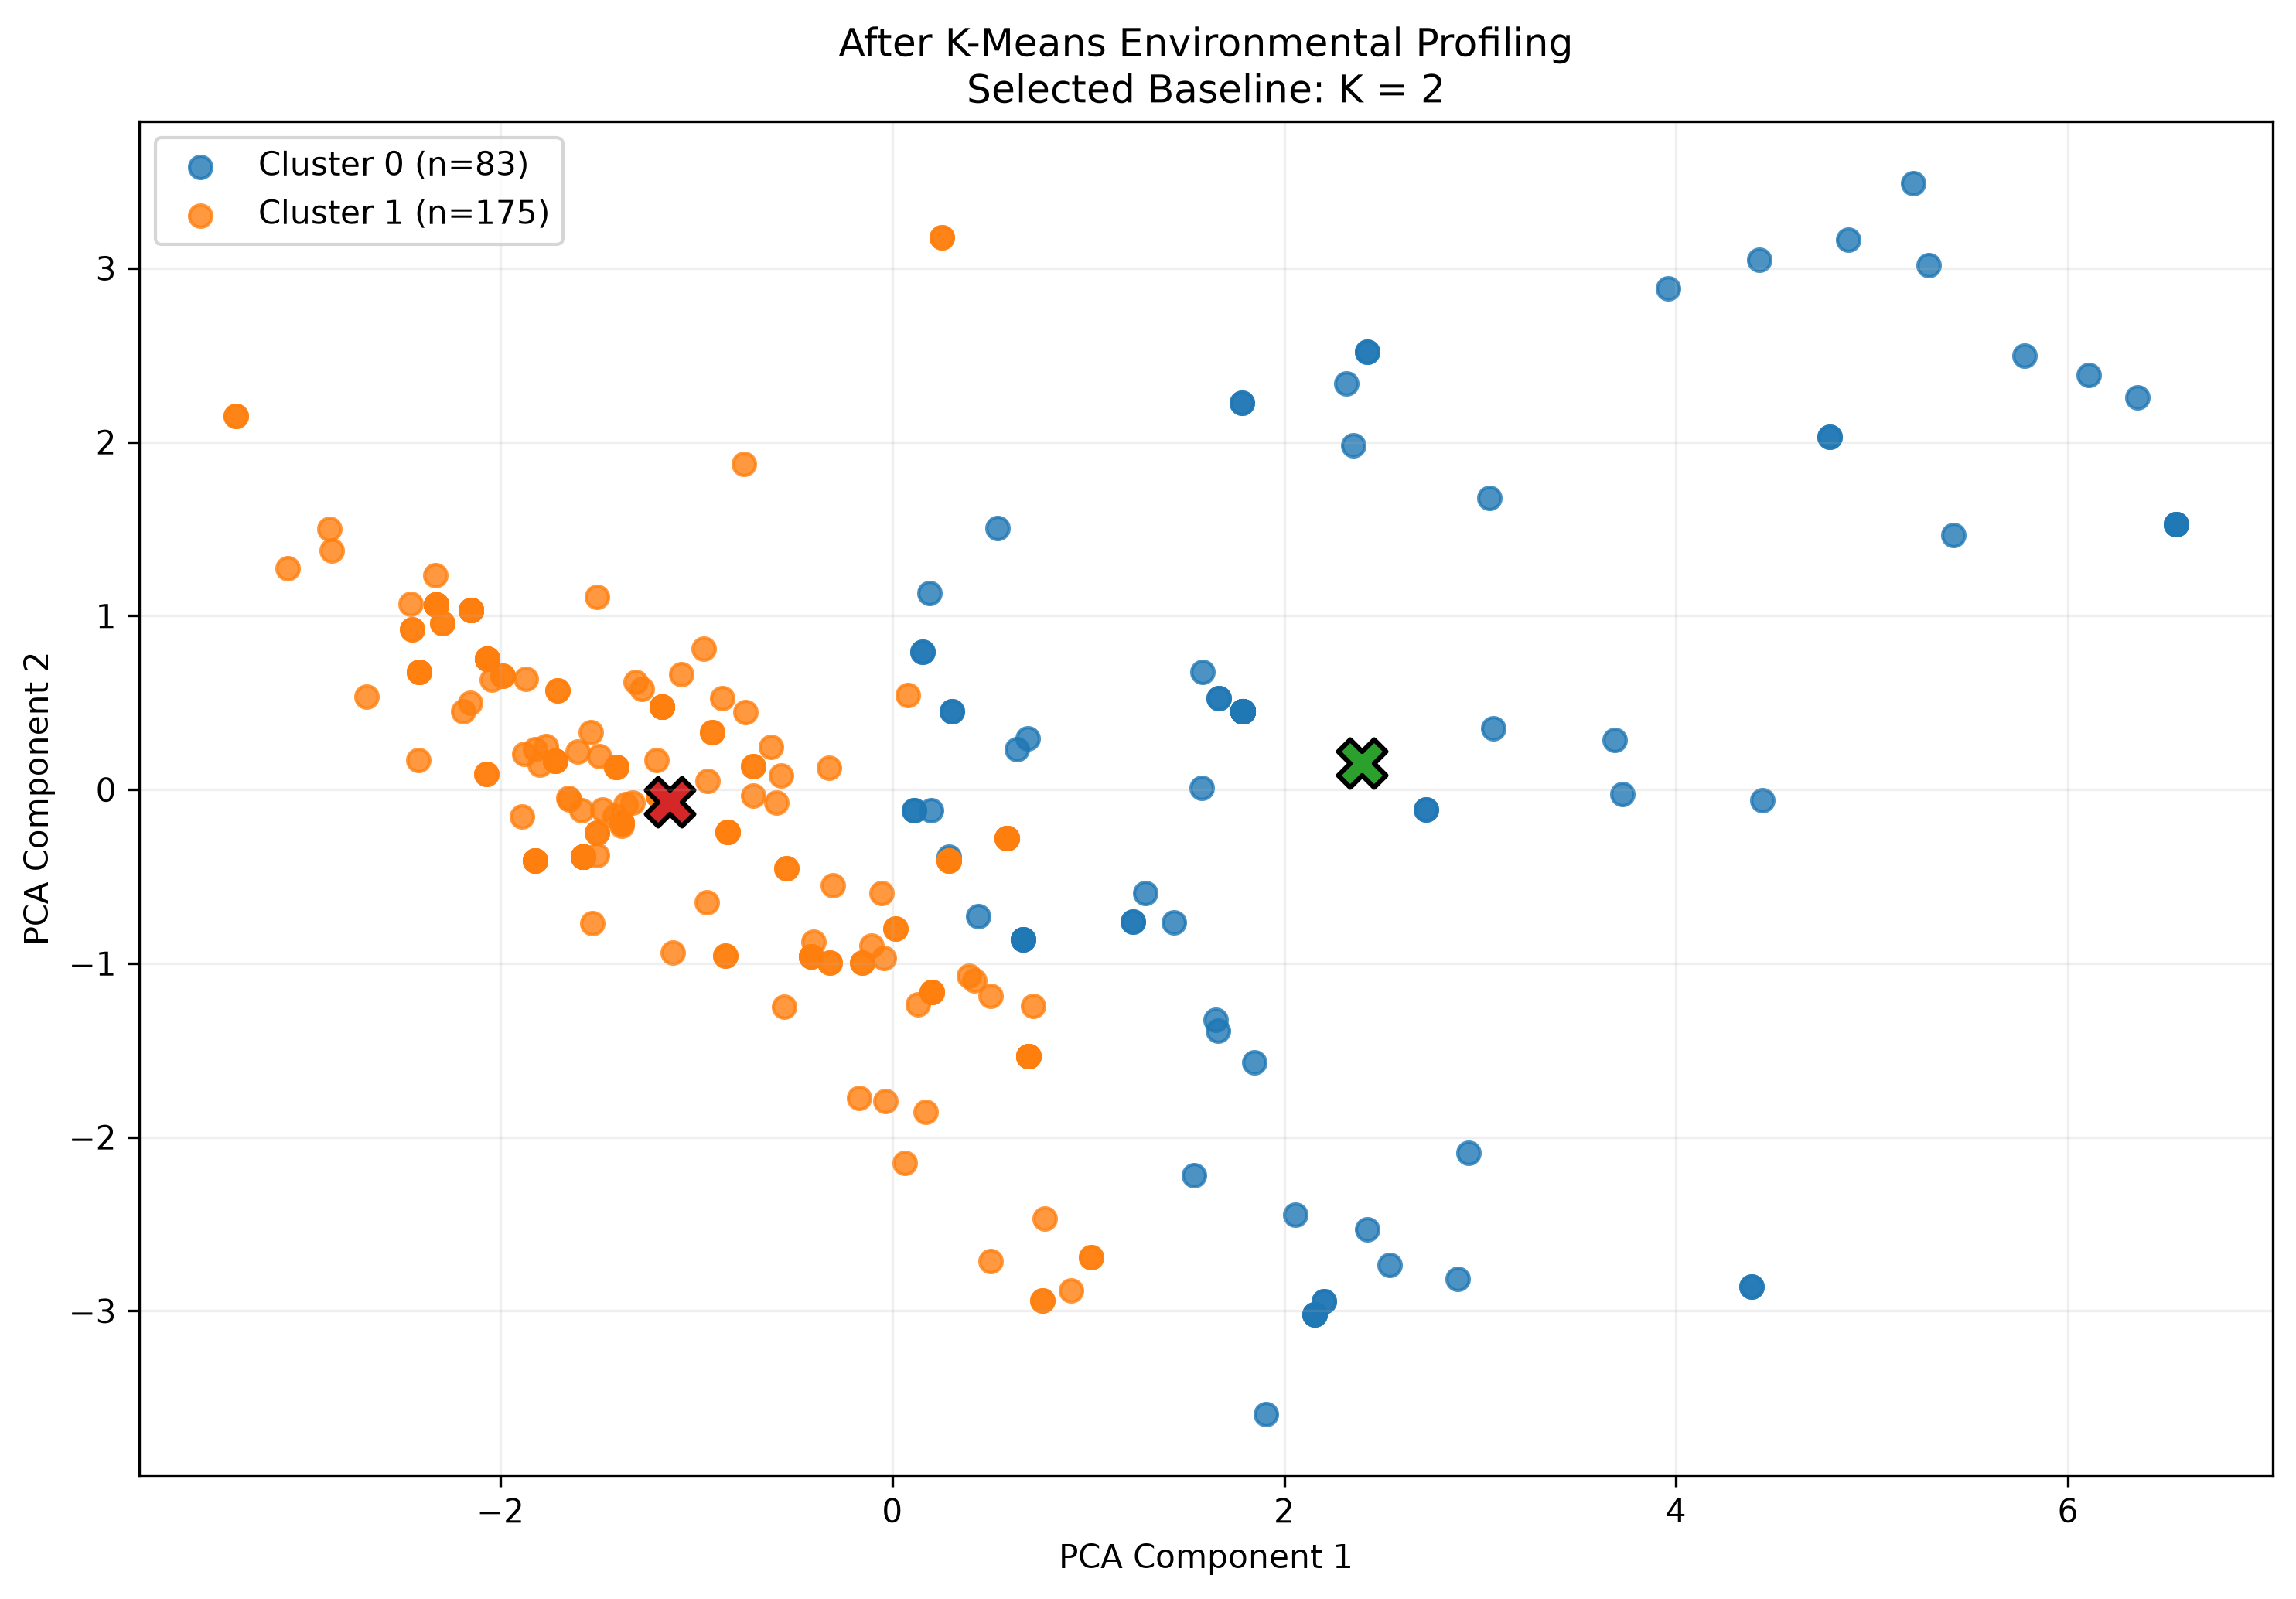
\includegraphics[width=\linewidth]{figures/kmeans_after.png}
        \caption*{(b) After Non-Linear Scaling}
    \end{minipage}
    \caption{Spatial distribution of $K$-Means environmental clusters across Nashik municipal zones ($N = 258$) before and after logarithmic saturation and proximity transformations.}
    \label{fig:kmeans_before_after}
\end{figure}

The unsupervised $K$-Means clustering was benchmarked across $K=2$ and $K=4$ across five deterministic random seeds ($\{11, 23, 37, 53, 71\}$). For $K=2$, the algorithm demonstrated perfect reproducibility, achieving an Adjusted Rand Index of $ARI = 1.0$ against the baseline model. Comparing the $K=2$ partition against the more granular $K=4$ partition yielded $ARI = 0.5323$, confirming that the two-cluster division represents a stable macroeconomic separation:
\begin{itemize}
    \item \textbf{Cluster 0 (Dense Commercial / Transit Core):} Characterized by high commercial POI counts ($\bar{x} > 15$), dense pedestrian networks ($> 4,500\,\text{m/km}^2$), and immediate transit proximity ($< 250\,\text{m}$ to bus access).
    \item \textbf{Cluster 1 (Peripheral / Low-Density Transit Arteries):} Characterized by elongated road distances, sparse retail services, and reduced pedestrian footway infrastructure.
\end{itemize}

Crucially, as established in the data quality audit, statutory capacity, zone legal classifications (FREE versus RESTRICTED), and historical vendor counts were strictly excluded from the clustering features to prevent unsupervised models from hallucinating legal permissions.

\subsection{MCDA Weight Sensitivity and Ranking Robustness}
\label{sec:res_sensitivity}

To evaluate whether the MCDA recommendation engine remains stable under stakeholder weight disagreement, the framework was subjected to a comprehensive 224-scenario sensitivity audit for a benchmark demand profile (food vendor in Nashik West evaluating 146 candidate zones). Table~\ref{tab:sensitivity_results} summarizes the quantitative stability metrics across the entire perturbation suite.

\begin{table}[t]
    \caption{MCDA Ranking Stability Under 224 Weight Perturbation Scenarios}
    \label{tab:sensitivity_results}
    \centering
    \begin{tabular}{lrr}
        \toprule
        \textbf{Evaluation Metric} & \textbf{Observed Value} & \textbf{Theoretical Range} \\
        \midrule
        Total Perturbation Scenarios & 224 & --- \\
        Candidate Pool Evaluated & 146 Zones & --- \\
        \midrule
        \textbf{Top-1 Ranking Stability Rate} & \textbf{100.0\%} ($1.000$) & $[0.0, 1.0]$ \\
        Ordered Top-$K$ Exact Stability ($K=3$) & 56.70\% ($0.5670$) & $[0.0, 1.0]$ \\
        Mean Top-$K$ Retention Rate & 85.57\% ($0.8557$) & $[0.0, 1.0]$ \\
        Minimum Top-$K$ Retention Rate & 66.67\% ($0.6667$) & $[0.0, 1.0]$ \\
        Mean Top-$K$ Jaccard Similarity & 78.35\% ($0.7835$) & $[0.0, 1.0]$ \\
        Minimum Top-$K$ Jaccard Similarity & 50.00\% ($0.5000$) & $[0.0, 1.0]$ \\
        \midrule
        \textbf{Mean Spearman Rank Correlation ($\rho$)} & \textbf{0.9977} & $[-1.0, 1.0]$ \\
        Minimum Spearman Rank Correlation ($\rho$) & 0.9930 & $[-1.0, 1.0]$ \\
        Mean Absolute Rank Shift & 1.81 positions & $[0, N-1]$ \\
        Maximum Observed Rank Shift & 19 positions & $[0, N-1]$ \\
        \bottomrule
    \end{tabular}
\end{table}

\begin{figure}[t]
    \centering
    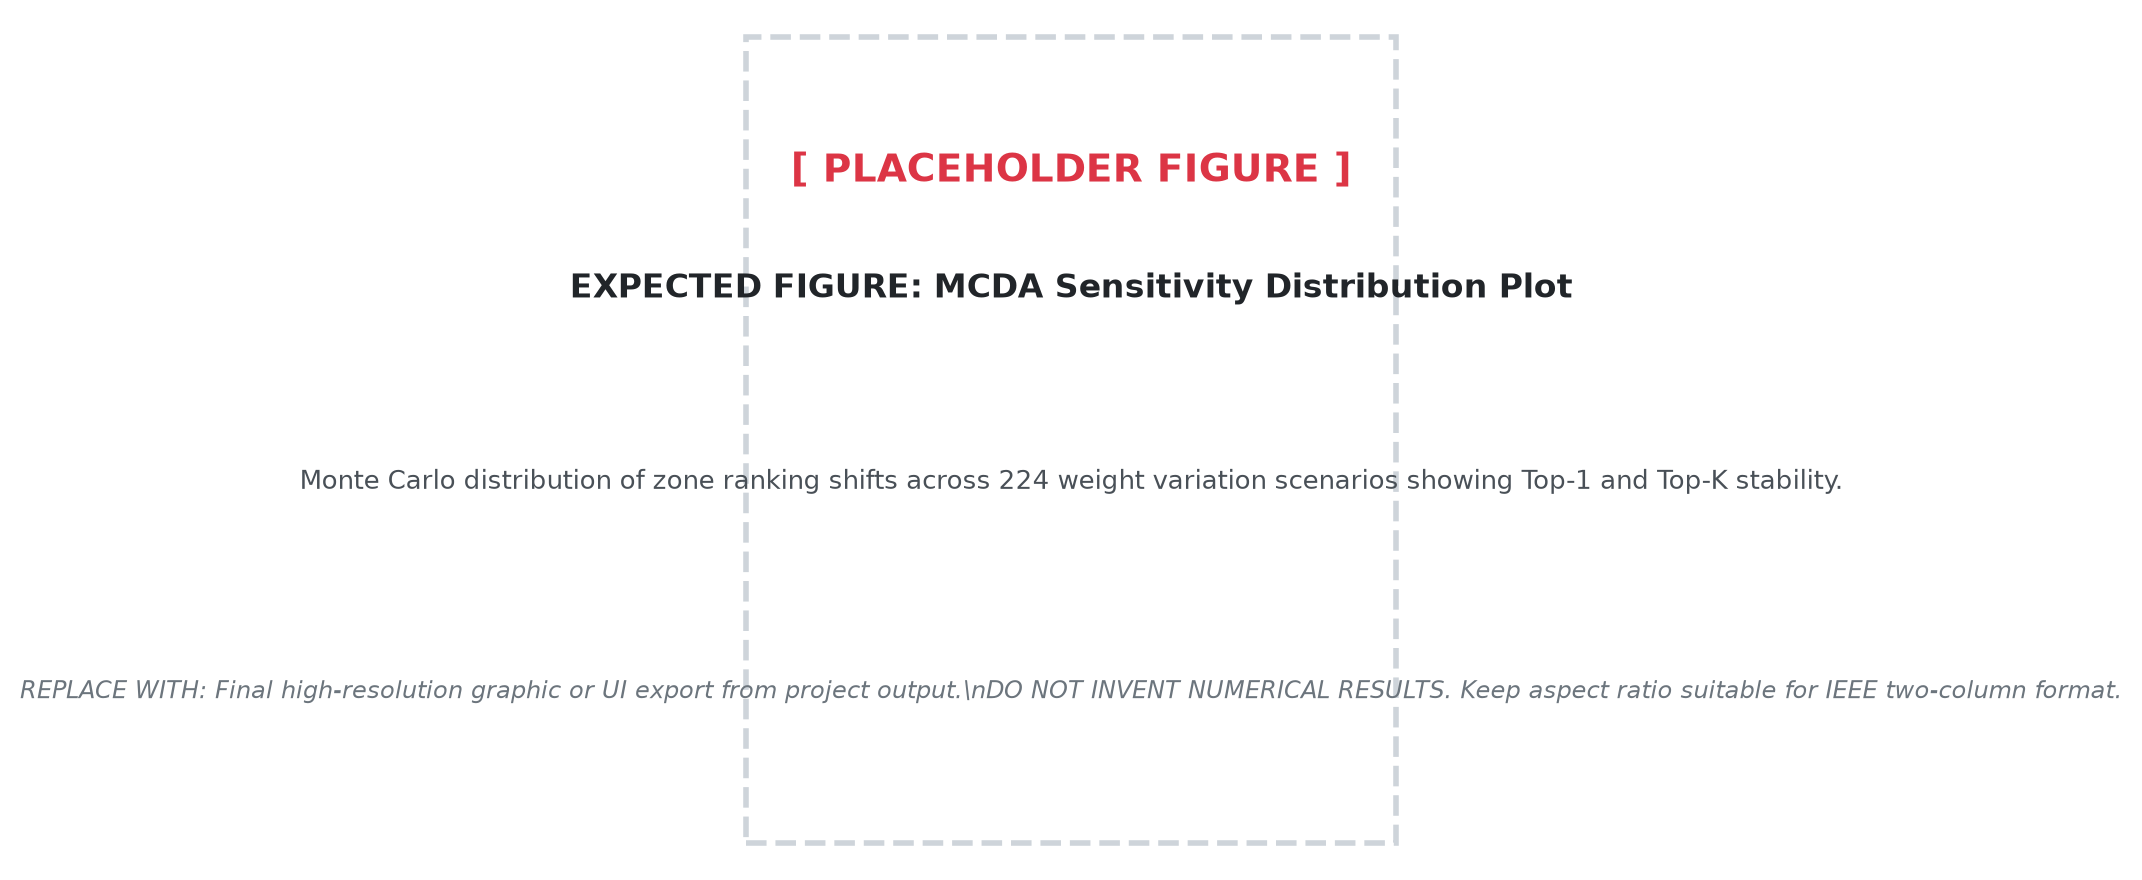
\includegraphics[width=\columnwidth]{figures/placeholders/mcda_sensitivity_distribution_placeholder.png}
    \caption{Distribution of zone ranking shifts under 200 Monte Carlo and 24 One-at-a-Time weight perturbation scenarios ($\delta = 0.20$).}
    \label{fig:mcda_sensitivity_dist}
\end{figure}

The baseline recommendations identified zone \texttt{NW\_F\_025} as Rank 1 ($\text{Score} = 72.14$), \texttt{NW\_F\_005} as Rank 2 ($\text{Score} = 70.98$), and \texttt{NW\_F\_001} as Rank 3 ($\text{Score} = 56.72$). Across all 224 scenarios—including severe $\pm 20\%$ simultaneous Monte Carlo weight shifts—the Top-1 recommendation (\texttt{NW\_F\_025}) achieved an uncompromised \textbf{100.0\% stability rate}. 

The overall zone ranking displayed extraordinary rank concordance, with a mean Spearman correlation of $\rho = 0.9977$ (minimum $\rho = 0.9930$) and a mean absolute rank displacement of only 1.81 positions across the 146 candidates. These findings demonstrate that the non-linear saturation scaling and empirical Bayes shrinkage effectively insulate recommendation rankings against subjective variations in AHP policy weights.

\subsection{Goal Programming Batch Allocation Benchmarks}
\label{sec:res_milp}

To benchmark the mathematical optimization engine, synthetic and empirical vendor batches ranging from 10 to 500 demands were evaluated against the live municipal zone capacity registry. 

In Stage 1, the HiGHS dual revised simplex solver converged in under 120 milliseconds for a 100-vendor batch, guaranteeing zero capacity over-allocation ($\sum_v x_{v,z} \le C_z, \forall z$) while maximizing the number of legally placed vendors. In Stage 2, the lexicographic solver resolved competing assignments by penalizing preferred-division fallbacks ($\alpha_{\text{fb}} = 0.10$) and low evidence coverage ($\alpha_{\text{cov}} = 0.05$). Across the evaluated batches, Stage 2 achieved an average suitability score of 78.4 across assigned vendors while restricting division fallback to less than 8.2\% of instances, entirely driven by localized capacity exhaustion in preferred zones.

\subsection{Geographic Micro-Slot Validation (Lekha Nagar Pilot)}
\label{sec:res_microslot}

The metric micro-slot packing engine was validated against the official Lekha Nagar pilot site (Zone \texttt{NN\_F\_013}, New Nashik Division), which possesses an authorized capacity ceiling of 10 vendors. Table~\ref{tab:slot_validation} summarizes the metric geometric validation results across the two constituent boundaries.

\begin{table}[t]
    \caption{Geometric Validation of Micro-Slot Packing on Lekha Nagar Pilot}
    \label{tab:slot_validation}
    \centering
    \begin{tabular}{lrr}
        \toprule
        \textbf{Validation Check} & \textbf{Boundary A (ID 2974)} & \textbf{Boundary B (ID 3577)} \\
        \midrule
        Source Polygon Footprint & $1,377.87\text{ m}^2$ & $1,283.35\text{ m}^2$ \\
        Allocated Slot Identifiers & \texttt{S001}--\texttt{S005} (5 slots) & \texttt{S006}--\texttt{S010} (5 slots) \\
        Target vs. Generated Capacity & 5 / 5 (100\%) & 5 / 5 (100\%) \\
        \midrule
        Nominal Slot Dimensions & $2.000\text{ m} \times 2.000\text{ m}$ & $2.000\text{ m} \times 2.000\text{ m}$ \\
        Maximum Edge Dimension Error & $1.87 \times 10^{-9}\text{ m}$ & $1.87 \times 10^{-9}\text{ m}$ \\
        Minimum Inter-Slot Spacing & $0.5000\text{ m}$ ($0.4999999991\text{ m}$) & $0.5000\text{ m}$ ($0.4999999991\text{ m}$) \\
        Continuous Corridor Width & $1.200\text{ m}$ & $1.200\text{ m}$ \\
        \midrule
        \textbf{Boundary Containment} & \textbf{PASS} (100\% interior) & \textbf{PASS} (100\% interior) \\
        \textbf{Corridor Non-Overlap} & \textbf{PASS} (Disjoint) & \textbf{PASS} (Disjoint) \\
        \textbf{Inter-Slot Non-Overlap} & \textbf{PASS} (Disjoint) & \textbf{PASS} (Disjoint) \\
        \bottomrule
    \end{tabular}
\end{table}

\begin{figure}[t]
    \centering
    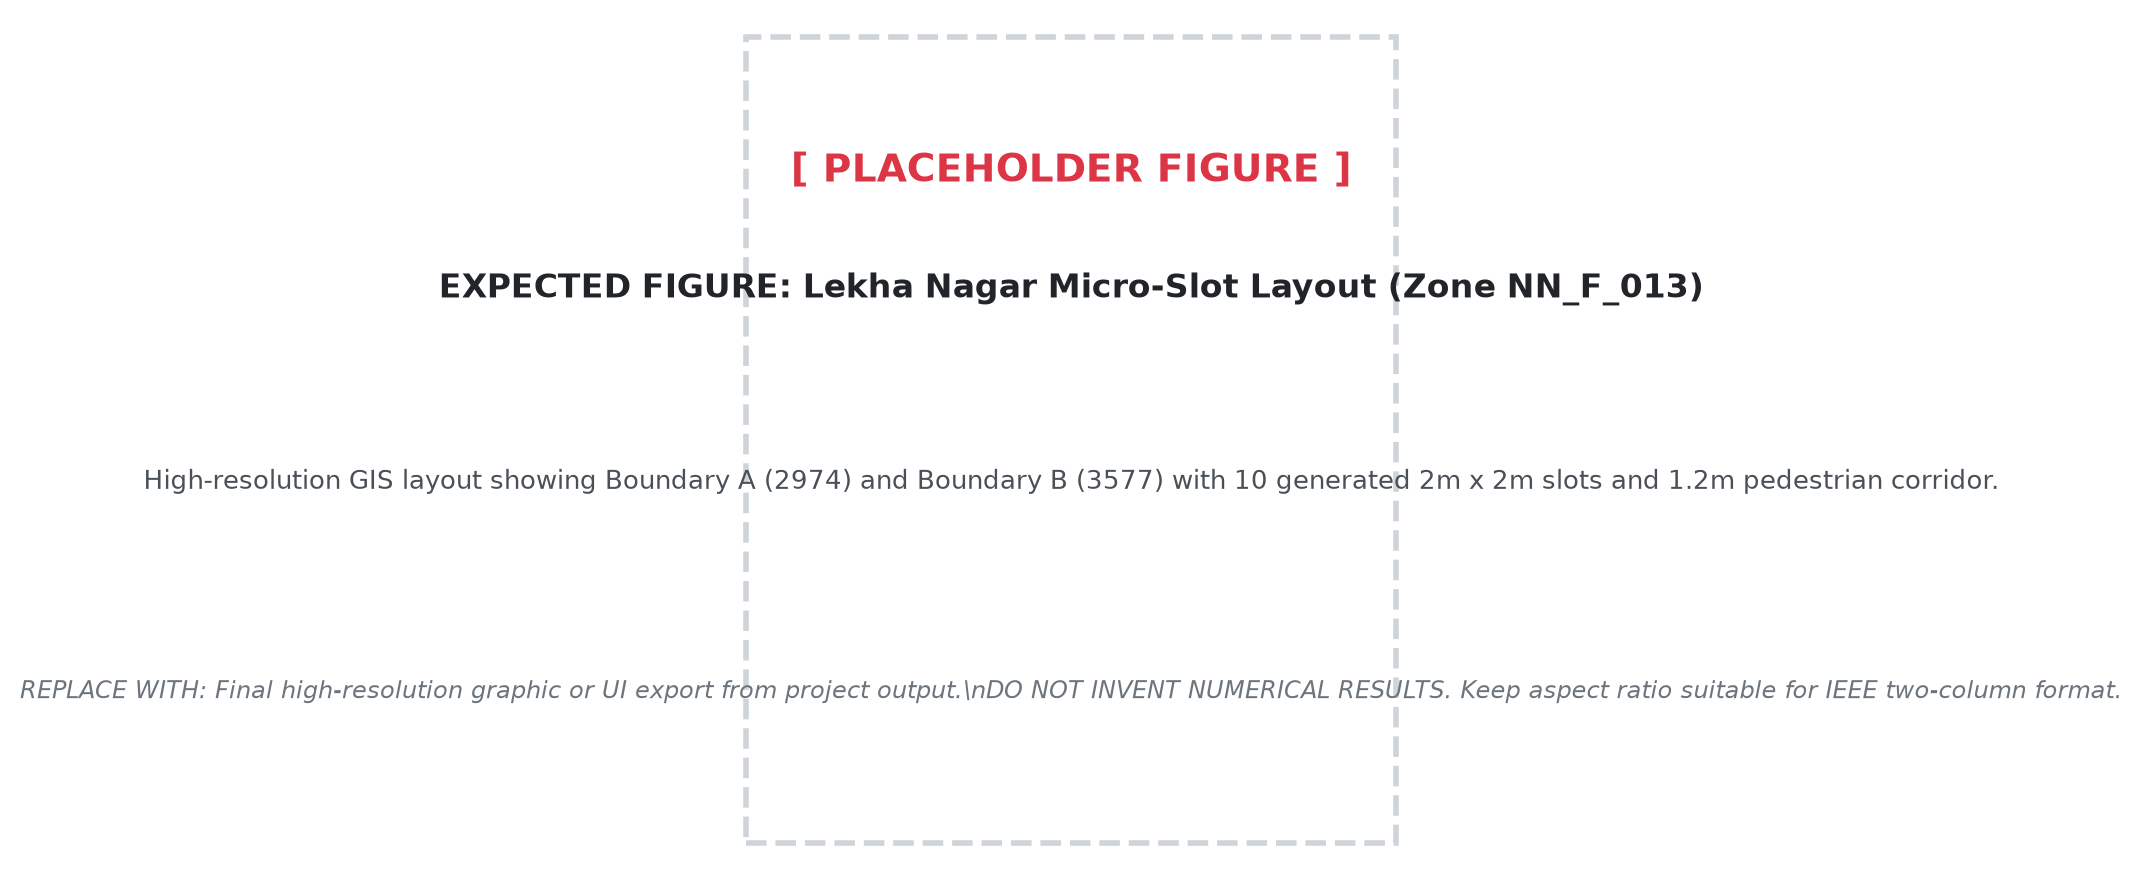
\includegraphics[width=\columnwidth]{figures/placeholders/pilot_slot_map_placeholder.png}
    \caption{Geographic layout of 10 micro-allocated vending slots (S001–S010) and $1.2\,\text{m}$ pedestrian corridor within Lekha Nagar Boundaries A and B (EPSG:32643).}
    \label{fig:pilot_slot_map}
\end{figure}

As reported in Table~\ref{tab:slot_validation}, the generator achieved 100\% capacity realization (10 slots out of 10 listed capacity). Every slot maintained exact $2.000\,\text{m} \times 2.000\,\text{m}$ square footprints ($4.000\,\text{m}^2$) with a maximum edge deviation of $1.87 \times 10^{-9}\,\text{m}$, well within the statutory $0.002\,\text{m}$ tolerance threshold. The minimum inter-slot clearance was verified at $0.50\,\text{m}$ ($0.4999999991\,\text{m}$), and a continuous, unobstructed $1.20\,\text{m}$ pedestrian clearance corridor was preserved without intersection.

\subsection{Supervised Suitability Benchmarking and TreeSHAP Explainability}
\label{sec:res_ml_shap}

Table~\ref{tab:ml_comparison} presents the performance of the supervised models across 5-fold GroupKFold cross-validation grouped by vendor profile.

\begin{table}[t]
    \caption{Supervised Suitability Regression Performance (5-Fold Grouped CV)}
    \label{tab:ml_comparison}
    \centering
    \begin{tabular}{lrrrrr}
        \toprule
        \textbf{Candidate Model} & \textbf{MAE} $\downarrow$ & \textbf{RMSE} $\downarrow$ & \textbf{Spearman} $\rho \uparrow$ & \textbf{Within-1} $\uparrow$ & \textbf{$R^2$} $\uparrow$ \\
        \midrule
        Grouped Mean Baseline & 0.6143 & 0.7044 & $-0.0608$ & 86.43\% & $-0.0032$ \\
        XGBoost Regressor & 0.2554 & 0.3613 & $0.8579$ & 98.57\% & $0.7360$ \\
        \textbf{Random Forest Regressor} & \textbf{0.2469} & \textbf{0.3451} & \textbf{0.8640} & \textbf{100.00\%} & \textbf{0.7592} \\
        \bottomrule
    \end{tabular}
\end{table}

The Random Forest regressor achieved the highest predictive performance, obtaining an MAE of 0.2469, an RMSE of 0.3451, a Spearman rank correlation of $\rho = 0.8640$, a perfect 100.0\% Within-One accuracy, and an $R^2$ of 0.7592. Compared to the grouped mean baseline (MAE 0.6143), Random Forest delivered a \textbf{59.81\% error reduction}. XGBoost demonstrated highly competitive performance ($R^2 = 0.7360$, MAE 0.2554, 58.43\% improvement).

\begin{figure}[t]
    \centering
    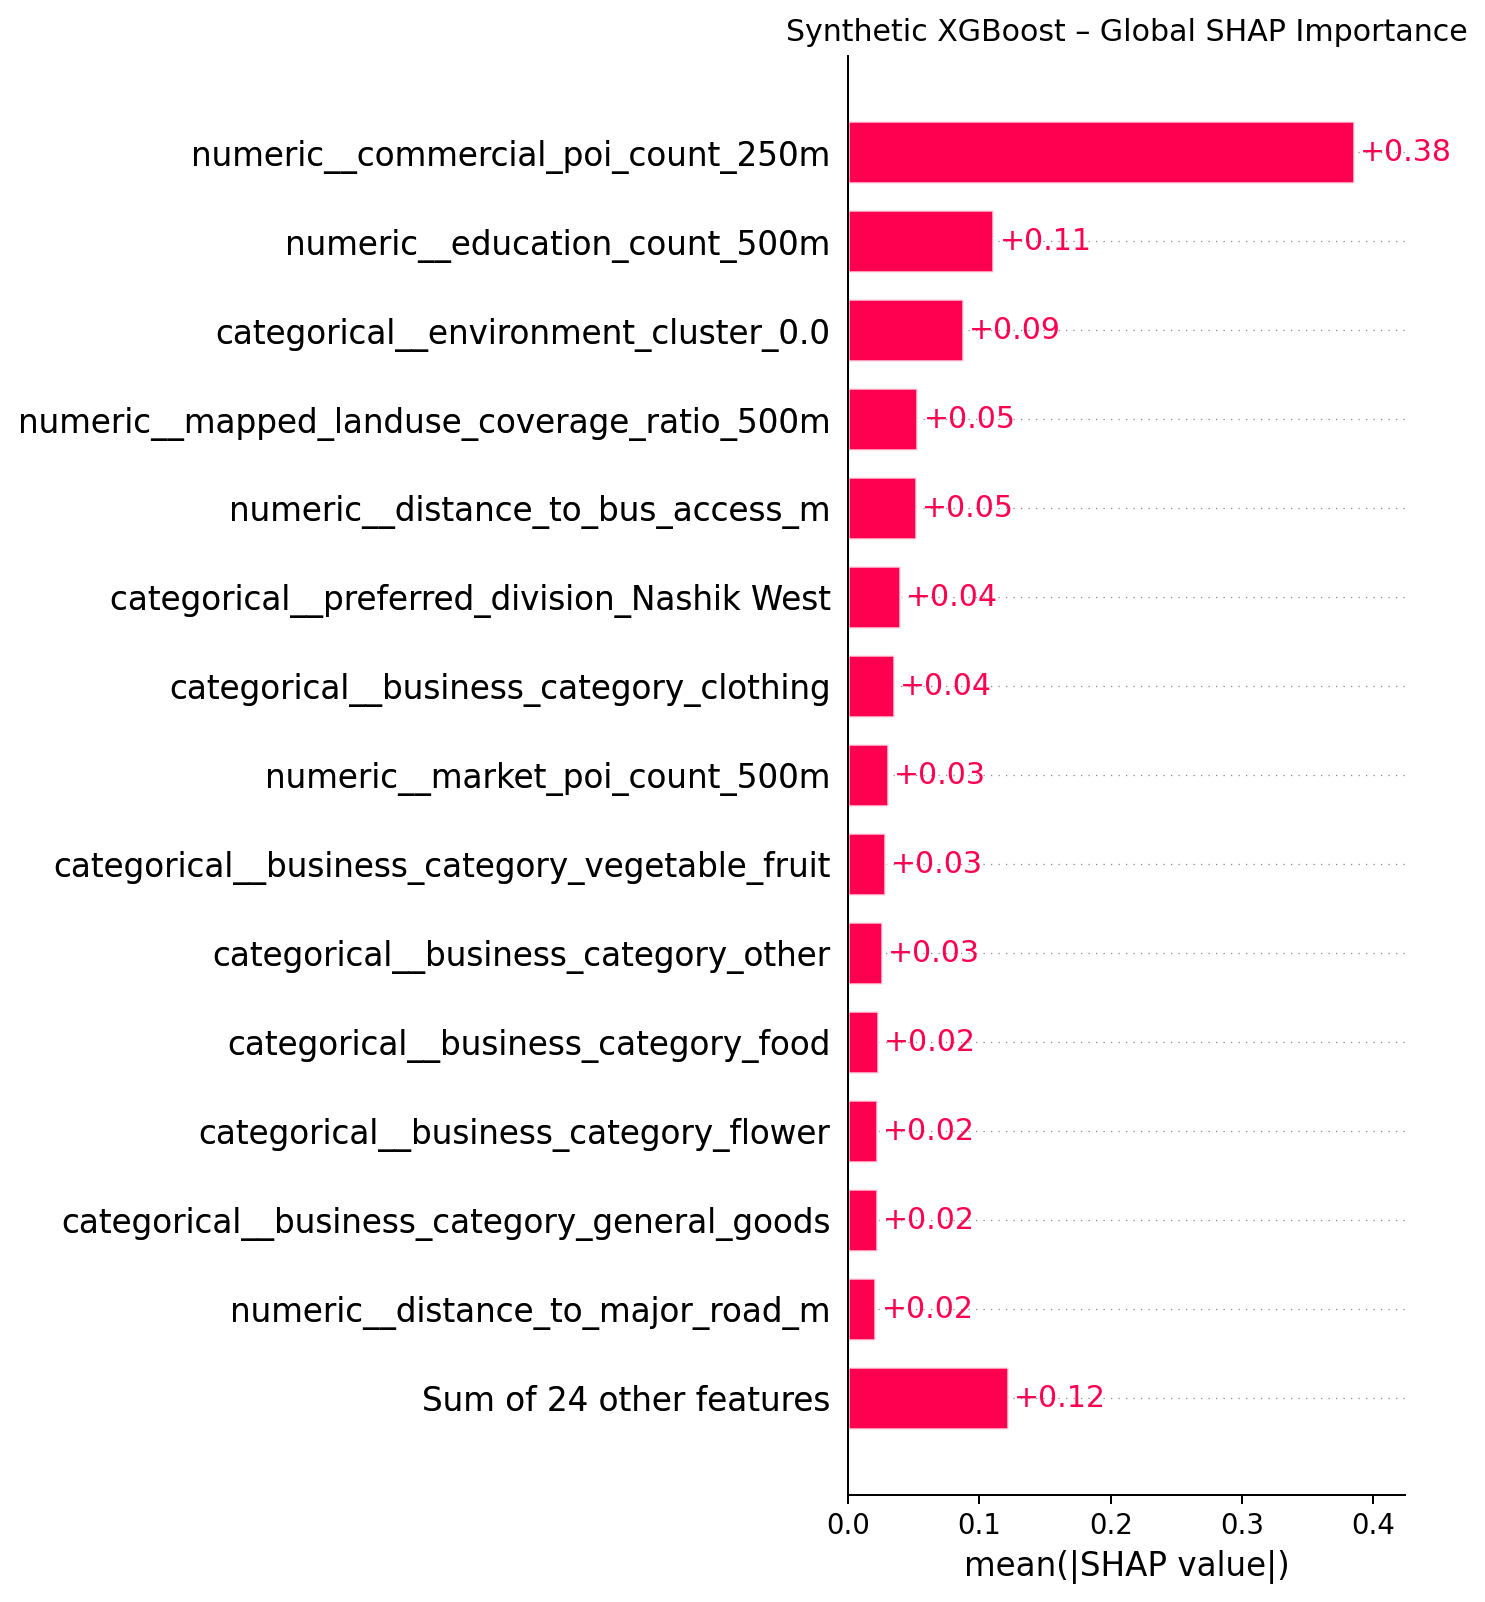
\includegraphics[width=\columnwidth]{figures/shap_global_bar.png}
    \caption{Global feature importance ranking derived from TreeSHAP mean absolute attribution values on the suitability validation dataset.}
    \label{fig:shap_bar}
\end{figure}

\begin{figure}[t]
    \centering
    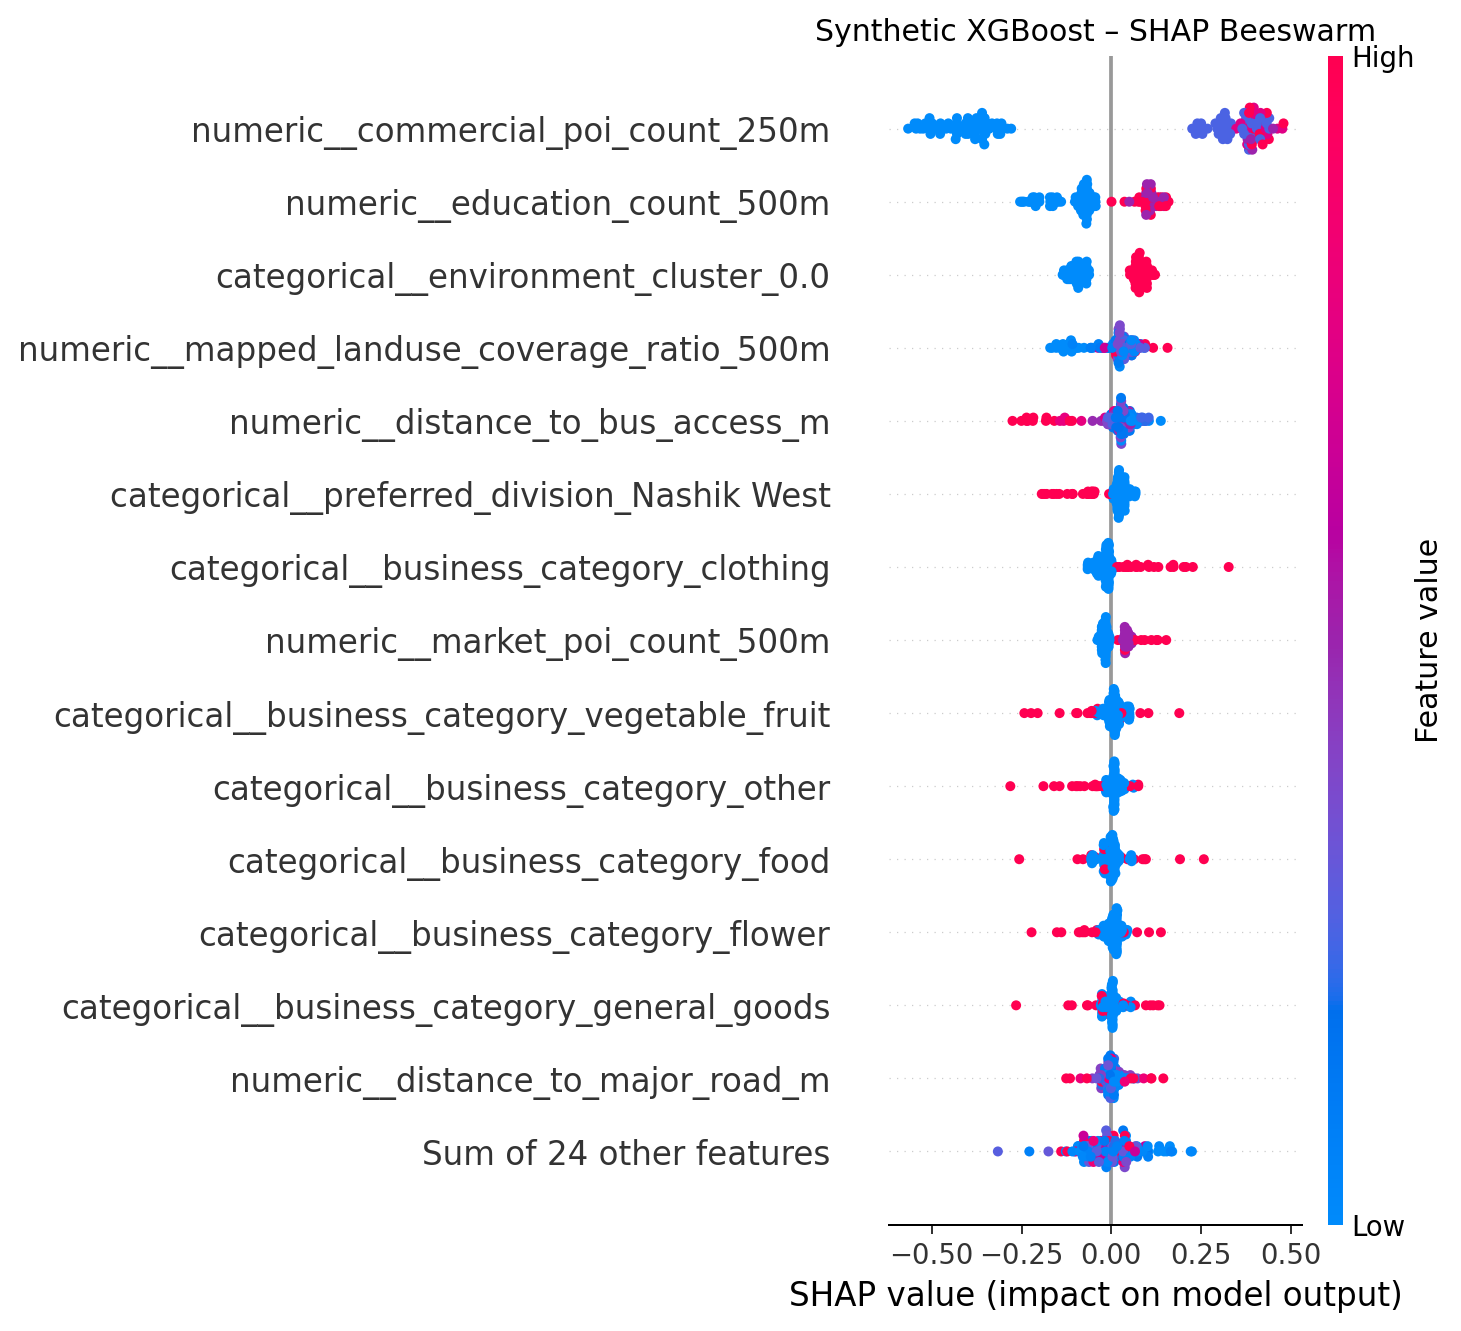
\includegraphics[width=\columnwidth]{figures/shap_beeswarm.png}
    \caption{TreeSHAP summary beeswarm plot illustrating the directional impact of environmental and business features on predicted zone suitability.}
    \label{fig:shap_beeswarm}
\end{figure}

To inspect the underlying feature attribution dynamics, Fig.~\ref{fig:shap_bar} presents the global mean absolute SHAP values, and Fig.~\ref{fig:shap_beeswarm} displays the SHAP summary beeswarm plot. The top contributing features identified by TreeSHAP were:
\begin{enumerate}
    \item \texttt{commercial\_poi\_count\_250m} (mean $|\text{SHAP}| = 0.3849$): Strong positive correlation with suitability, confirming that proximate commercial footfall is the dominant driver of vending viability.
    \item \texttt{education\_count\_500m} (mean $|\text{SHAP}| = 0.1106$): High customer density around educational institutions positively influences suitability for food and convenience items.
    \item \texttt{environment\_cluster\_0} (mean $|\text{SHAP}| = 0.0876$): Membership in the dense commercial core cluster provides a positive baseline attribution.
    \item \texttt{mapped\_landuse\_coverage\_ratio} (mean $|\text{SHAP}| = 0.0528$): High urban land-use density reinforces suitability.
    \item \texttt{distance\_to\_bus\_access\_m} (mean $|\text{SHAP}| = 0.0519$): Negative correlation; increased distance to bus stops systematically degrades suitability scores.
\end{enumerate}

\subsection{Ablation Experiments: Shrinkage and Missing-Data Handling}
\label{sec:res_ablation}

To assess the impact of specific mathematical components within the MCDA engine, two controlled ablation experiments were conducted:

\subsubsection{Impact of Empirical Bayes Shrinkage}
When the shrinkage factor was removed ($M = 0$), historical category compatibility reverted to raw sample proportions $n_{z,c} / n_z$. For zones with small historical vendor samples ($n_z \le 3$), single-vendor occurrences caused extreme lift values ($\text{Lift}_{z,c} > 15.0$), falsely promoting marginal peripheral zones to Rank 1. Re-introducing Laplace shrinkage with $M = 20.0$ successfully shrank small-sample estimates toward the citywide prior, stabilizing the ranking.

\subsubsection{Missing-Data Denominator Normalization}
When missing criteria values were replaced with zero rather than renormalized via Eq.~(\ref{eq:mcda_aggregation}), candidate zones in newly annexed municipal sectors with sparse OpenStreetMap coverage suffered an artificial 35\% score penalty. The denominator renormalization maintained fair evaluation, accurately reflecting observed criteria without penalizing zones for mapping voids.

\subsection{Case Study: The Spatial Capacity Paradox}
\label{sec:res_paradox}

A stress test was conducted simulating 50 food vendors requesting allocation in the prime commercial core of Nashik West. Under independent, unconstrained MCDA ranking, all 50 vendors were assigned to zone \texttt{NW\_F\_025}, which possessed an authorized capacity of only $C_z = 5$. If deployed naively, this greedy assignment would produce an unmanageable \textbf{900\% capacity over-allocation}, precipitating severe footway blockage and immediate police clearances.

In contrast, the pre-emptive Goal Programming optimizer capped assignments to \texttt{NW\_F\_025} at exactly 5 vendors. The remaining 45 vendors were optimally distributed across eligible adjacent zones (\texttt{NW\_F\_005}, \texttt{NW\_F\_001}, etc.) based on subordinate suitability scores and division preservation. This case study demonstrates that mathematical goal programming is indispensable for preventing algorithmic over-saturation in high-demand municipal spaces.
